\begin{enumerate}[label=\thechapter.\arabic*,ref=\thechapter.\theenumi]

\item Consider the differential equation $\frac{d^2y}{dx^2}-2\frac{dy}{dx}+y=0$. The boundary conditions are $y=0$ and $\frac{dy}{dx}=1$ at $x=0$. Then the value of $y$ at $x=\frac{1}{2}$ \hfill (GATE AE 2022)\\
\solution
\iffalse
\let\negmedspace\undefined
\let\negthickspace\undefined
\documentclass[journal,12pt,twocolumn]{IEEEtran}
\usepackage{cite}
\usepackage{amsmath,amssymb,amsfonts,amsthm}
\usepackage{algorithmic}
\usepackage{graphicx}
\usepackage{textcomp}
\usepackage{xcolor}
\usepackage{txfonts}
\usepackage{listings}
\usepackage{enumitem}
\usepackage{mathtools}
\usepackage{gensymb}
\usepackage{comment}
\usepackage[breaklinks=true]{hyperref}
\usepackage{tkz-euclide} 
\usepackage{listings}
\usepackage{gvv}                                        
\def\inputGnumericTable{}                                 
\usepackage[latin1]{inputenc}                                
\usepackage{color}                                            
\usepackage{array}                                            
\usepackage{longtable}                                       
\usepackage{calc}                                             
\usepackage{multirow}                                         
\usepackage{hhline}                                           
\usepackage{ifthen}                                           
\usepackage{lscape}
\newtheorem{theorem}{Theorem}[section]
\newtheorem{problem}{Problem}
\newtheorem{proposition}{Proposition}[section]
\newtheorem{lemma}{Lemma}[section]
\newtheorem{corollary}[theorem]{Corollary}
\newtheorem{example}{Example}[section]
\newtheorem{definition}[problem]{Definition}
\newcommand{\BEQA}{\begin{eqnarray}}
\newcommand{\EEQA}{\end{eqnarray}}
\newcommand{\define}{\stackrel{\triangle}{=}}
\theoremstyle{remark}
\newtheorem{rem}{Remark}
\begin{document}

\bibliographystyle{IEEEtran}
\vspace{3cm}

\title{GATE: AE - 37.2022}
\author{EE23BTECH11224 - Sri Krishna Prabhas Yadla$^{*}$% <-this % stops a space
}
\maketitle
\newpage
\bigskip

\renewcommand{\thefigure}{\arabic{figure}}
\renewcommand{\thetable}{\arabic{table}}


\vspace{3cm}
\textbf{Question:} Consider the differential equation $\frac{d^2y}{dx^2}-2\frac{dy}{dx}+y=0$. The boundary conditions are $y=0$ and $\frac{dy}{dx}=1$ at $x=0$. Then the value of $y$ at $x=\frac{1}{2}$ \hfill (GATE AE 2022)\\
\solution
\fi
\begin{table}[htbp]
	\centering
	\def\arraystretch{1.5}
	\begin{tabular}{|c|c|c|}
\hline
\textbf{Parameters} & \textbf{Values} & \textbf{Description} \\
\hline
$y(0)$ & 0 & $y$ at $x=0$\\
\hline
$y'(0)$& 1 &$\frac{dy}{dx}$ at $x=0$ \\
\hline
\end{tabular}

	\caption{Parameters}
	\label{tab:parameters}
\end{table}
\begin{align}
\label{L(y'')}\frac{d^2y}{dx^2} &\system{L} s^2Y(s)-sy(0)-y'(0)\\
\label{L(y')}\frac{dy}{dx} &\system{L} sY(s)-y(0)
\end{align}
Applying Laplace Transform, using \eqref{L(y'')} and \eqref{L(y')},
\begin{align}
s^2Y(s)-sy(0)-y'(0) - 2(sY(s)-y(0)) + Y(s) = 0
\end{align}
From \tabref{tab:parameters},
\begin{align}
(s^2-2s+1)Y(s)-1 &= 0 \\
Y(s) &= \frac{1}{(s-1)^2}\\
\label{L(t^n)}t^n &\system{L} \frac{n!}{s^{n+1}}\\
	\label{complex_shift}e^{at} x(t) &\system{L} X(s-a)
\end{align}
Taking Inverse Laplace Transform for $Y(s)$, using \eqref{L(t^n)} and \eqref{complex_shift},
\begin{align}
y(x) &= xe^x \\
\implies y\brak{\frac{1}{2}} &= \frac{\sqrt{e}}{2}
\end{align}
\begin{figure}[htbp]
	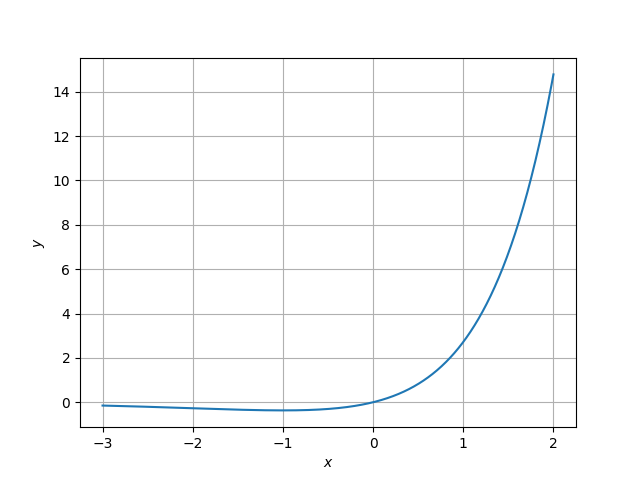
\includegraphics[width=\columnwidth]{2022/AE/37/figs/plot.png}
	\caption{Plot of $y(x)$}
	\label{fig:plot}
\end{figure}


\pagebreak
\end{enumerate}
